\documentclass{article}
\usepackage{qilin}
\tikzstyle{process} = [rectangle, rounded corners, minimum width=1.5cm, minimum height=0.5cm,align=center, draw=black, fill=gray!30, auto]
\title{ECE360: Electronics}
\author{QiLin Xue}  
\date{Fall 2022}
\usepackage{mathrsfs}
\usetikzlibrary{arrows}
\usepackage{stmaryrd}
\usepackage{accents}
\newcommand{\ubar}[1]{\underaccent{\bar}{#1}}
\usepackage{pgfplots}
\numberwithin{equation}{section}
\usetikzlibrary{quantikz}
\usepackage[american]{circuitikz}
\newcommand{\equals}{=}

\begin{document}

\maketitle
\tableofcontents
\newpage
\section{Diodes}
A \emf{diode} is an electronic valve that allows current to flow in one direction.
\begin{center}
    \begin{circuitikz}
        \draw (2,0) to [D] (0,0); 
    \end{circuitikz}
\end{center}
The cathode is the vertical line and typically corresponding to a black strip on the physical diode, and the triangle is the anode. Current can only flow in the direction of the arrow. Diodes are an example of a \emf{two-terminal device,} which only has a single voltage and a single current.

The \emf{ideal diode} has the following properties:
\begin{itemize}
    \item Acts as a short-circuit when ON or conducting
    \item Acts as an open-circuit when OFF or not conducting
\end{itemize}
One of the most common uses is a \emf{Half-wave rectifier,} which is used for generating a DC signal from a pure AC signal...
\begin{center}
    \begin{circuitikz}
        \draw[] (0,0)node[ground]{} to [sV=$v_s$] (0,2) to [D] (2,2) to [R] (2,0) to (0,0);
    \end{circuitikz}
\end{center}
The AC source would produce a sinusoidal pattern. If $v_s > 0,$ the diode is ON, and the voltage drop across the resistor is $v_0=v_S.$ IF $v_s < 0,$ the diode is OFF and the voltage drop across the resistor is $v_0=0.$ 

A diode is an example of a \emf{non-linear} component, meaning that we cannot use our standard tools of circuit analysis. Instead, we need to \textit{assume} a state, \textit{analyze} the circuit, then \textit{verify} it. A helpful tool, is by looking at the graph of current against voltage:
\begin{center}
    \begin{tikzpicture}
    \begin{axis}[
    legend pos=outer north east,
    title=Current Against Voltage,
    axis lines = middle,
    xlabel = $v$,
    ylabel = $i$,
    variable = t,
    trig format plots = rad,
    yticklabels={,,},
    xticklabels={,,},
    ]
    \addplot [
        domain=-7:7,
        samples=70,
        color=blue,
        style=ultra thick
        ]
        {x};
    \addlegendentry{resistor}
    \addplot [
        domain=-7:0,
        samples=70,
        color=red,
        style=ultra thick
        ]
        {0};
    \addplot [
        domain=0:0.0001,
        samples=70,
        color=red,
        style=ultra thick
        ]
        {5/0.0001*x};
    \addlegendentry{diode} 
    \end{axis}
    \end{tikzpicture}
\end{center}
\newpage
\begin{example}
    \begin{center}
        \begin{circuitikz}
            \draw[] (0,0)node[ground]{} to [V,v=$v_2$,invert] (0,2) to [D] (2,2) to (4,2) node[right] {$v_0$};
            \draw[] (-2,2)node[ground]{} to [V=$v_1$,invert](-2,4) to [D=$D_1$] (3,4) to (3,2) to [R=$R$] (3,0)node[ground]{};
        \end{circuitikz}
    \end{center}
    which can be described by the table
    \begin{center}
        \begin{tabular}{ccccc}
            $V_1$ & $D_1$ & $V_2$ & $D_2$ & $V_0$ \\
            5V    & ON    & 5V    & ON    & 5V    \\
            5V    & ON    & 0V    & OFF   & 5V    \\
            0V    & OFF   & 5V    & ON    & 5V    \\
            0V    & OFF   & 0V    & OFF   & 0V   
            \end{tabular}
    \end{center}
    which represents an OR gate.
\end{example}
\begin{example}
    Suppose we wish to find the output voltage $v_0$
    \begin{center}
        \begin{circuitikz}
            \draw[] (0,0)node[ground]{} to (1,0) to [D=$D_1$](1,-2) to [R=$R_1\equals 10\text{ k}\Omega$](1,-4)node[below]{$-10V$};
            \draw[] (1,-2) to (4,-2) to [D=$D_2$,invert](4,0) to [R=$R_2 \equals 5\text{ k}\Omega$](4,2)node[above]{$10V$};
            \draw [] (4,0) to (5,0)node[right]{$v_0$};
        \end{circuitikz}
    \end{center}
    Suppose both diodes are ON, i.e. they act as short circuits. Then $v_0=0V.$ However, if we compute the currents through $D_1$ and $D_2,$ we'll see that $D_1$ has current flowing in the opposite direction! This means that we have to repeat, assume a different diode configuration, and verify again.
    \vspace{2mm}

    If the right diode was ON, then the current through both resistors would be $1.33\text{ mA},$ setting $v_0 = 3.33\text{ V}.$ The voltage across the left diode is negative, so everything agrees.
\end{example}
\subsection{Terminal Characteristics of a PN-Junction}
In an actual PN-junction, there are three regions we will discuss, highlighted in yellow below. However, in this course, we will only be focusing on the forward and reverse regions.
\begin{center}
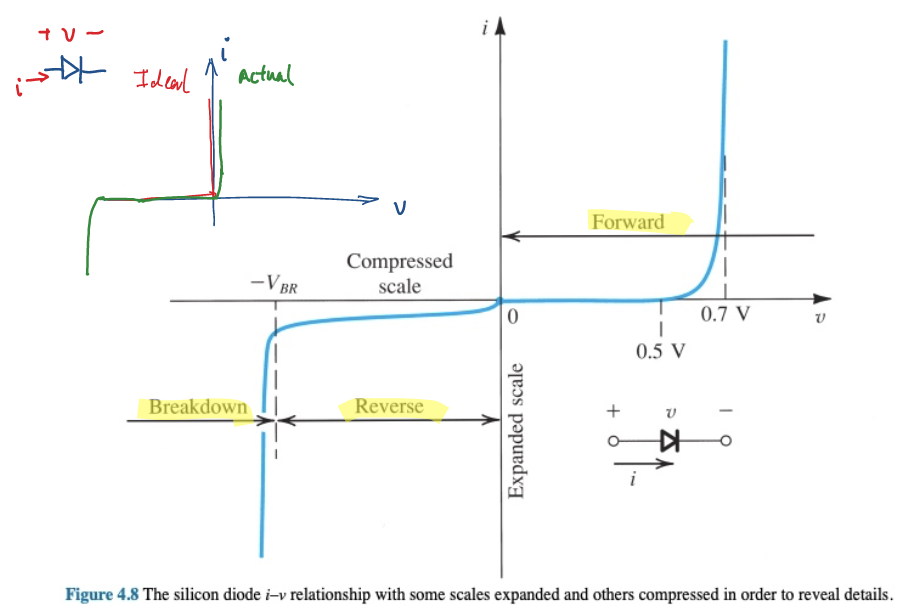
\includegraphics[width=0.9\linewidth]{silicon diode.png}
\end{center}
\emf{Forward Bias ($v>0$):} The current has an exponential relationship, given by
\begin{equation}
    i = I_s\left(e^{v/v_T} - 1\right),
\end{equation}
where $v_T$ is the \emf{thermal voltage,} given by
\begin{equation}
    v_T = \frac{kT}{q} \approx 25\text{ mV}
\end{equation}
where $k$ is Boltzmann's constant, $T$ is the temperature, and $q$ is the charge of an electron. $I_s$ is the \emf{saturation current,} which is a tiny number (on the scale of nanoamperes). The saturation current doubles roughly every $+5^\circ \text{C}$ increase in temperature and is proportional to the cross-section of the diode. Because $v \gg v_T$ typically, we can ignore the $-1$ constant. This means we can write the voltage drop as
\begin{equation*}
    v = v_T\ln(i/I_s) = 2.303v_T\log(i/I_s).
\end{equation*}
Suppose we have two diodes where the currents are $i_1,i_2$ and voltages are $v_1,v_2.$ Then:
\begin{align*}
    \frac{i_2}{i_1} &= e^{\frac{v_2-v_1}{v_T}} \\ 
    v_2 - v_1 &= v_T\ln\left(i_2/i_1\right)  = (60\text{ mV})\log(i_2/i_1).
\end{align*}
Writing everything in terms of logarithms is important in practice and engineering because we are often  interested in the \textit{order of magnitude} of currents and voltages.

\emf{Temperature Dependence:}
\begin{itemize}
    \item At constant current, the voltage drop decreases by approximately $2\text{ mV}$ for every $1^\circ\text{C}$ increase in temperature.
    \item $I_S$ doubles roughly every $5^\circ\text{C}$ increase in temperature.
\end{itemize}
\emf{Reverse Bias ($v<0$):} Since $v \ll v_T,$ the exponential term can be ignored, and we have a constant:
\begin{equation*}
    i = - I_S.
\end{equation*}
Note that the actual reverse current is much larger than the saturation current. For example, $i_\text{reverse}=-1\text{ nA}$ when $I_S = -1\text{ pA}.$
\begin{example}
    Calculate the diode voltage and current in the circuit below. Assume that the diode voltage is $0.7\text{ V}$ at $1\text{ mA}$ and $v_T = 25\text{ mV}.$
    \begin{center}
        \begin{circuitikz}
            \draw[](0,0) to [V=$5V$, invert] (0,2) to [D=$D_1$, l=$V_D$] (3,2) to [R=$1\text{ k}\Omega$](3,0) to (0,0);
        \end{circuitikz}
    \end{center}
    Using the above information, we have:
    \begin{align*}
        & 1\text{ mA}  = I_se^{(0.7V)/(25mV)} \\ 
        \implies & I_s = 6.9\times 10^{-16}\text{ A}.
    \end{align*}
    The current through the diode is
    \begin{align*}
        I_D = I_Se^{V_D/v_T}
    \end{align*}
    And Kirchoff's Loop Rule gives us
    \begin{align*}
        5-V_D = I_DR.
    \end{align*}
    Solving this using a graphing calculator, we get 
    \begin{align*}
        I_D &= 4.264\text{ mA} \\ 
        V_D &= 0.736\text{ V}.
    \end{align*}
    We can also use an iterative solution. Recall that 
    \begin{align*}
        v - v_0 = v_T\ln\left(\frac{i}{i_0}\right),
    \end{align*}
    where we are given $v_0=0.7V$ and $i_0=1\text{ mA}.$
    \vspace{2mm}

    We can guess $v_1 = 0.5V,$ which gives $i_1 = 4.5\text{ mA}.$ Using this new current, we can compute $v_2=0.738V,$ and get the current to be $i_2 = 4.262\text{ mA}.$ In general:

    \begin{align*}
        v_{n+1} &= v_0 + v_T\ln\left(\frac{i_n}{i_0}\right) \\ 
        i_{n+1} &= \frac{5-v_{n+1}}{R}
    \end{align*}
\end{example}
We can build a simpler model of the diode, called the \emf{Constant Voltage Drop} (CVD) model, which is the same as an ideal diode, except the graph is shifted $0.7V$ to the right. That is, if the voltage drop is lower than $0.7V,$ the diode will be closed, otherwise the voltage drop is $0.7V$ and current is able to flow through freely.

Another model is the \emf{small signal model.} There are certain problems where the diode is in the forward bias region, but is operating in a very small range. In this case, we can approximate the diode as a linear resistor, with a voltage drop of $0.7V.$ This is a good approximation for small signal diodes, but is not accurate for large signal diodes.
\newpage
\begin{example}
    Find the variation on the diode voltage given the supply is $V_{dd}=5V\pm 0.5V.$
    \begin{center}
        \begin{circuitikz}
            \draw[](0,0) to [V=$5V$, invert] (0,2) to [D=$D_1$, l=$V_D$] (3,2) to [R=$1\text{ k}\Omega$](3,0) to (0,0);
        \end{circuitikz}
    \end{center}
    We've already computed that $V_D=0.736V$ when $V_S=5V.$ We can compute $V_{S,max}=0.739V$ and $V_{S,min}=0.736V.$ But computing these numbers without a computer is difficult (since we want precision). Instead, we can use a small signal model, which approximates the diode as a resistor and a voltage source.
    \vspace{2mm}

    Specifically, we can write $V_S=5\text{ V}$ as our operating point, and $v_{\mathcal{S}}$, allowing us to draw,
    \begin{center}
        \begin{circuitikz}
            \draw[](0,0) to [V=$V_S\equals 5V$, invert] (0,2) 
            to [sV,l=$v_{\mathcal{S}}\equals 0.5V$] (0,4)
            to [R, l=$1\text{ k}\Omega$] (3,4) to [V=$V_{dd}$](6,4)
            to [R=$r_d$](6,0) to (0,0);
        \end{circuitikz}
    \end{center}
    Using our above information, we can compute $r_d = 5.8\Omega,$ so 
    \begin{equation*}
        v_d = \frac{r_d}{R+r_d} \times v_{\mathcal{S}} = \pm 3\text{ mV}
    \end{equation*}
\end{example}
\section{Clamping Circuits}
\subsection{Clamped Capacitor Circuits}
\begin{center}
    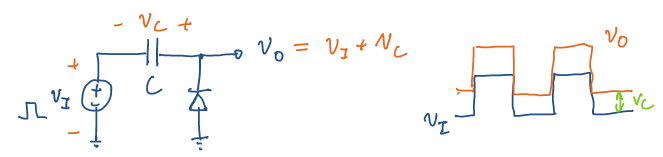
\includegraphics[width=0.8\linewidth]{clamped capacitor.png}
\end{center}
\href{https://www.falstad.com/circuit/circuitjs.html?ctz=CQAgjCAMB0l3BWcMBMcUHYMGZIA4UA2ATmIxAUgpABZsKBTAWjDACgB3EPKsQ3-uEGQ2AYyECqaPBKhRYEJjWg1INYtgTE+CbBgIyRXabJQJCskQHMQZi7hq3zIbGjkiAJk-trvpkB4MAGYAhgCuADYALpx+fFSaKJZsAG7cUhhJPJbgtFRIVIXQCGw22ZhZCb6FbAD2coSOVKqkyPJJVBYJ1PkuubwubEA}{Example}
\subsection{Peak Detector}
\begin{center}
    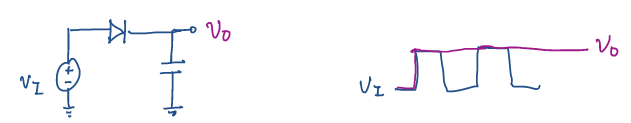
\includegraphics[width=0.8\linewidth]{peak detector.png}
\end{center}
\subsection{Voltage Doubler}
This is very useful because we can generate a voltage higher than the source that we can supply.
\begin{center}
    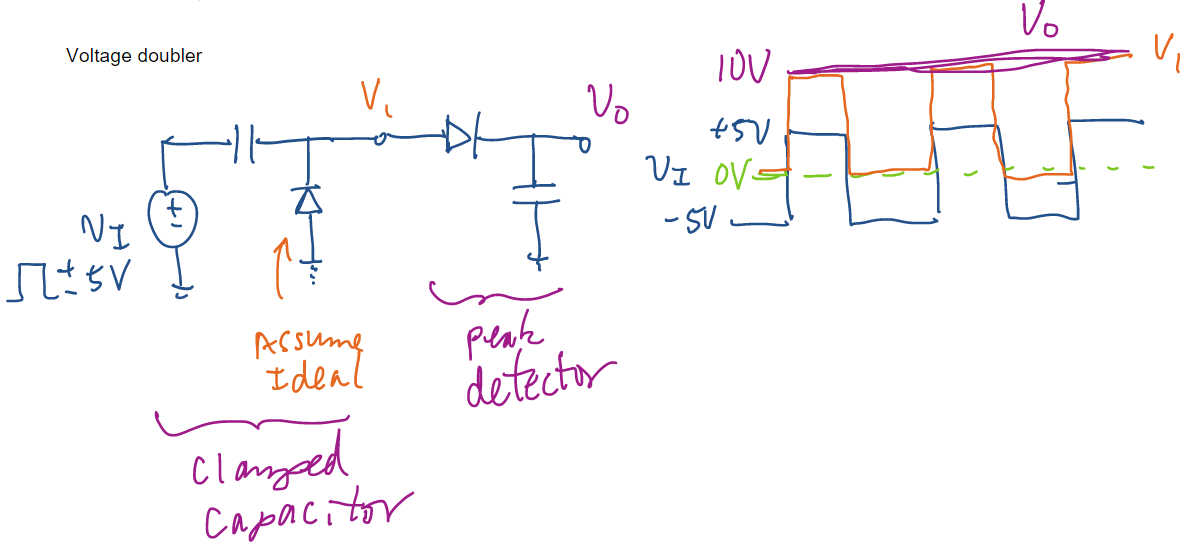
\includegraphics[width=0.8\linewidth]{voltage doubler.png}
\end{center}
\section{Breakdown Region}
After a certain voltage is sustained across the diode in reverse bias, it can break down (avalanche effect). \emf{Zener diodes} operate in this region and are often represented as a constant voltage source of $V_z = 5V.$
\end{document}